\documentclass[a4paper,draft]{article}

\usepackage[utf8]{inputenc}
\usepackage[T1]{fontenc}

\usepackage{lmodern}
\usepackage{amsmath}
\usepackage{amssymb}
\usepackage{stmaryrd}

\usepackage{mathtools}
\usepackage{amsthm}
\usepackage{thmtools}
\declaretheorem{lemma}
\declaretheorem[style=definition,qed=$\blacktriangle$]{example}
\declaretheorem[style=definition,qed=$\blacktriangle$]{definition}
\numberwithin{equation}{section}

\usepackage{enumitem}
\setlist[enumerate,1]{label=\alph*)}
\newlist{prfcases}{enumerate}{1}
\setlist[prfcases,1]{label={\it Case \arabic*.},align=left,leftmargin=\parindent,itemindent=*}

\usepackage{algorithm}

\usepackage{tikz}
\usetikzlibrary{shapes.geometric}
\tikzset{itermtree/.style={level distance=6mm,sibling distance=10mm,%
	edge from parent/.style={draw,solid},every node/.style={solid}}}
\tikzset{pure/.style={draw,rectangle,inner sep=4pt,minimum size=5mm}}
\tikzset{term/.style={draw,circle,inner sep=1pt,minimum size=5mm}}
\tikzset{ap/.style={fill,diamond,inner sep=0pt,minimum size=6pt}}
\tikzset{subtrm/.style={draw,isosceles triangle,isosceles triangle apex angle=55,%
	shape border rotate=90,minimum height=10mm,anchor=north,child anchor=north}}
\tikzset{subtrmf/.style={subtrm,level distance=10mm,sibling distance=16.67mm}}
\tikzset{subtrmn/.style={subtrm,level distance=4mm,sibling distance=6.67mm}}
\tikzset{abbrv/.style={dashed}}

\usepackage[
	style=numeric,
	sorting=none,
	doi=false,
	urldate=iso8601,
]{biblatex}
\addbibresource{bibliography.bib}

\usepackage[hidelinks]{hyperref}


\newcommand{\ldb}{\llbracket}
\newcommand{\rdb}{\rrbracket}
\newcommand{\todo}{\fbox{To do.}}

\newcommand{\oftype}{\mathrel{::}}
\newcommand{\funT}{\Rightarrow}
\newcommand{\abs}[2]{\lambda #1.\>#2}
\newcommand{\All}[2]{\bigwedge #1.\>#2}
\newcommand{\all}[2]{\forall #1.\>#2}
\newcommand{\set}[2]{\{#1\mid #2\}}

\DeclareMathOperator{\pure}{\mathit{pure}}
\newcommand{\ap}{\diamond}
\DeclareMathOperator{\sterm}{\mathsf{term}}
\DeclareMathOperator{\spure}{\mathsf{pure}}
\newcommand{\sap}{\mathbin{\mathsf{`ap`}}}
\newcommand{\sapp}{\>}
\newcommand{\sabs}[2]{{\boldsymbol\lambda} #1.\>#2}
\newcommand{\termeq}{=_{\alpha\beta\eta}}


\title{Applicative Functors in Isabelle/HOL: Notes}
\author{Joshua Schneider}

\begin{document}

\maketitle
\section{Project Overview}\label{sec:overview}

\subsection{Introduction}\label{subsec:introduction}

Our primary goal is to implement an Isabelle/HOL proof method which reduces
lifted equations to their base form.
% FIXME restriction to Isabelle/HOL?
Here, lifting refers to a transition from operations on base types to related
operations on some structure.
Hinze~\cite{hinze10} studied the conditions under which lifting preserves the
validity of equations.
He noticed that lifting can be defined in an intuitive fashion if the target
structure is an applicative functor~\cite{mcbride08}:
a unary type constructor $f$ with associated constants%
\footnote{Types are given in Isabelle notation.}
\begin{align*}
	\pure_f &\oftype \alpha \funT \alpha f, \\
	(\ap_f) &\oftype (\alpha \funT \beta) f \funT \alpha f \funT \beta f.
\end{align*}
The operator $\ap_f$ is left-associative.
We omit the subscripts if the functor is clear from the context.
Moreover, the following laws must be satisfied:
\begin{align*}
	\tag{identity} \pure{\mathit{id}} \ap u &= u \\
	\tag{composition} \pure{(\cdot)} \ap u \ap v \ap w &= u \ap (v \ap w) \\
	\tag{homomorphism} \pure{f} \ap \pure x &= \pure{(f x)} \\
	\tag{interchange} u \ap \pure{x} &= \pure{(\abs{f}{f x})} \ap u
\end{align*}

The identity type constructor defined by $\alpha\,\mathit{id} = \alpha$ is a
trivial applicative functor for $\pure{x} = x$, $f \ap x = f x$.
We can take any abstraction-free term $t$ and replace each constant $c$ by
$\pure{c}$, and each instance of function application $f x$ by $f \ap x$.
The rewritten term is equivalent to $t$ under the identity functor
interpretation, or identity ``idiom'' as coined in \cite{mcbride08}.
By choosing a different applicative functor, we obtain a different
interpretation of the same term structure.
In fact, this is how we define the lifting of $t$ to an idiom.
We also permit variables, which remain as such in the lifted term, but range
over the structure instead.
A term consisting only of $\pure$ and $\ap$ applications and
free variables is called an idiomatic expression.

\begin{example}\label{exmp:set-intro}
Another applicative functor can be constructed from sets.
For each type $\alpha$ there is a corresponding type $\alpha\,\mathit{set}$
of sets with elements in $\alpha$;
$\pure$ denotes the singleton set constructor $x \mapsto \{x\}$;
$F \ap X$ takes a set of functions $F$ and a set of arguments $X$
with compatible type, applying each function to each argument:
\[ F \ap X = \set{f x}{f \in F,\, x \in X}. \]
We can lift addition on natural numbers to the set idiom by defining the operator
\begin{align*}
	(\oplus) &\oftype \mathit{nat}\,\mathit{set} \funT \mathit{nat}\,\mathit{set} \funT
		\mathit{nat}\,\mathit{set}, \\
	X \oplus Y &= \pure{(+)} \ap X \ap Y = \set{x + y}{x \in X,\, y \in Y}.
\end{align*}
The associative property of addition
\[ \all{x y z}{(x + y) + z = x + (y + z)} \]
can be translated to sets of natural numbers
\[ \all{X Y Z}{(X \oplus Y) \oplus Z = X \oplus (Y \oplus Z)}, \]
where it holds as well, as one can check with a slightly laborious proof.
Note that the two sides of the latter equation are the lifted counterparts
of the former, respectively.
\end{example}

As we have seen, lifting can be generalized to equations.
There is actually a more fundamental relationship between the two equations
from above example---the lifted form can be proven for all applicative
functors, not just $\mathit{set}$, using only the base property and the
applicative functor laws.
We want to automate this step with a proof method.

Not all equations can be lifted in all idioms, though.
In certain cases stronger conditions are required.
\todo{}

\subsection{User Interface}\label{subsec:interface}

Since Isabelle's core logic does not allow parameterization of type constructors,
we need a custom mechanism for registering applicative functors with the
system.
In order to apply the proof method, the user must provide beforehand
\begin{enumerate}
	\item corresponding $\pure$ and $\ap$ instances, and
	\item a proof of the applicative functor laws, optionally with extended
	properties.
\end{enumerate}
Lifted constants may be registered with an attribute, which can be applied to
facts $\mathit{lhs} = \mathit{rhs}$, where $\mathit{rhs}$ is an idiomatic
expression.
These must be suitable for rewriting.

The complete set of subgoal forms to support has not been determined yet.
\todo{}
As a minimal requirement, after unfolding lifted constants, HOL equations of
idiomatic expressions shall be handled.
Only the outermost functor $f$ is considered per invocation.
The conceptual variables of the lifted expressions may be instantiated with
arbitrary terms.
However, the method actually proves the fully universally quantified form---%
for every subterm not matching $\pure_f{\_}$ or $\_ \ap_f \_$, a new, locally
quantified variable is introduced.
The method attempts to transform the first subgoal to the base form of the
equation, in other words, its identity functor interpretation.
Variable names shall be preserved, if possible.
Finally, it is desirable to have some kind of debugging facility for tracing
intermediate steps.

\begin{example}\label{exmp:set-usage}
Continuing with the set idiom from Example~\ref{exmp:set-intro}, assume that
the user wants to prove an instantiation of the associativity law for $\oplus$,
\[ (X \oplus Y) \oplus F a = X \oplus (Y \oplus F a), \]
as part of a larger proof, where $X$, $Y$ and $F$ are fixed variables, and
$a$ is a constant.
The system has been informed of $\mathit{set}$ and $\oplus$.
After applying the proof method, the new proof obligation reads
\[ \All{x y u}{(x + y) + u = x + (y + u)}. \qedhere \]
\end{example}

\subsection{Proof Strategy}\label{subsec:proof-strategy}

The proof method starts with testing the first subgoal for the expected
structure.
If the test succeeds, the applicative functor $f$ is known, such that the
relevant theorems can be accessed subsequently.
We then rewrite the subgoal using the declared rules for lifted constants.
Only those related to $f$ are used, the reason being that overeager, unwanted
unfolding may be difficult to reverse.
All following steps depend on which additional properties of $f$ have been
provided.

If there are none, we normalize both sides of the equation.
Hinze's Normal Form Lemma~\cite[7]{hinze10} asserts the existence of a certain
normal form for idiomatic expressions where each variable occurs only once.
As it turns out, we can compute this normal form for arbitrary terms.
This is convenient because opaque parts are handled implicitly.
The details of the normalization algorithm are described in Section~\ref{sec:normal-form}.
The normalized equation is
\[ \pure{g} \ap t_1 \ap \cdots \ap t_m = \pure{h} \ap s_1 \ap \cdots \ap s_n, \]
where $g$ and $h$ are new terms, and $\vec t$ and $\vec s$ are the opaque
subterms of the original equation.
If either $m \ne n$ or $t_i \ne s_i$ for some $i$ (as terms modulo
$\alpha\beta\eta$-conversion), the proof method fails.
Otherwise, we apply appropriate congruence rules until the subgoal is reduced
to $g = h$.
Since $g$ and $h$ are at least $n$-ary functions, we can further apply
extensionality, reaching the subgoal
\[ \All{x_1 \dots x_n}{g x_1 \cdots x_n = h x_1 \cdots x_n}. \]
The normal form has the interesting property that this is exactly the
generalized base form of the original equation.

\todo

\subsection{Choice of Embedding}\label{subsec:embedding}

In Isabelle, it is not possible to construct an abstract framework for
applicative functors in such a way that it is inhabited by all instances.
We already referred to the fact that type constructors are fixed.
Another issue is the lack of polymorphism in the inner logic:
We cannot have, say, a schematic variable \textit{?pure} and use it with
different types within the same proposition or proof.
One solution is to define a custom logic, including a term language, axioms
and meta theorems, and formalize it using the available specification tools.
This is a \emph{deep embedding}~\cite{wildmoser04} of the logic.
Then it would be possible to derive the Normal Form Lemma as a regular
inference rule, for example.
However, we want to prove propositions about arbitrary HOL objects, not just
their encodings in the embedded logic.
Some machinery is necessary, which performs the encoding and transfers results.
\begin{itemize}
\item finite number of types involved per term $\implies$ could use sum types
\item number of types in sum is linear in size of terms
\item would introduce a large number of projections/abstractions
\end{itemize}
\todo

A different approach, which we will take, is a \emph{shallow embedding}.
The ``formul\ae'' (here, idiomatic terms) are expressed directly in HOL.
Due to aforementioned restrictions, meta-theorectical results must be provided
in specialized form for each case.
We make use of the powerful ML interface of Isabelle to program the proof
construction.
The correctness of the proofs is still verified by the system, of course.

\section{Normal Form Conversion}\label{sec:normal-form}

McBride and Paterson~\cite{mcbride08} noted that idiomatic expressions can
be transformed into an application of a pure function to a sequence of impure
arguments.
They called this the \emph{canonical form} of the expression.
Hinze~\cite[Section~3.3]{hinze10} gave an explicit construction based on the
monoidal variant of applicative functors.  % TODO define somewhere
Transforming the terms in this way is useful for our purpose, because the
arguments of the remaining $\pure$ terms reflect the equation that was lifted.
The soundness of the algorithm depends only on the applicative laws, making it
the most general approach regarding functors (but not regarding lifted
equalities).
We will later show that all transformations based on the applicative laws yield
a unique canonical form, modulo $\alpha\beta\eta$-conversion.
Therefore, we follow Hinze and denote by \emph{normal form} this particular
canonical form.
The distinction is necessary, as we will consider other canonical forms in
Section~\ref{sec:combinators}, which are justified by additional laws.

In the following, we define lifting and normalization formally, based on a
syntactic representation of idiomatic terms.
While this presentation is more abstract than what is actually happening in
Isabelle, it makes it easier to demonstrate correctness and some other
properties.
Unlike Hinze, we use the $\pure$/$\ap$ formalism.
Then we describe the implementation of the normalization procedure in
Isabelle/ML.

\subsection{The Idiomatic Calculus}\label{subsec:idiomatic-calculus}

In Section~\ref{subsec:introduction}, we introduced idiomatic expressions built
from $\pure$ and $\ap$ constants of an applicative functor.
This structure maps straightforward to a recursive datatype, given that there
is a representation for arguments of $\pure$.
These must have some structure as well such that the applicative laws can be
expressed.
It should also be possible to have ``opaque'' idiomatic subterms, which cannot
(or should not) be written as a combination of $\pure$ and $\ap$.
This is primarily useful for variables ranging over lifted types, but as
demonstrated in Example~\ref{exmp:set-usage}, more complex terms may occur too.
Therefore it makes sense to refer to general lambda terms in both cases;
then we can define semantics consistently.
Types are ignored here for simplicity.
However, all results are compatible with the restrictions of simply typed
lambda calculus.

\begin{definition}[Untyped lambda terms]
Let $\mathcal{V}$ be an infinite set of variable symbols.
We assume that $f$, $g$, $x$, $y$ are disjoint variables in the following
formulas.
The set of untyped lambda terms is defined as
\begin{equation}
	\mathcal{T} ::= \mathcal{V} \mid (\mathcal{T} \sapp \mathcal{T}) \mid
		\sabs{\mathcal{V}}{\mathcal{T}}
\end{equation}
An equivalence relation on $\mathcal{T}$ is a $\mathcal{T}$-congruence iff it
is closed under application and abstraction.
Let $\termeq$ be the smallest $\mathcal{T}$-congruence containing $\alpha$-,
$\beta$-, and $\eta$-conversion.
\end{definition}

\begin{definition}[Idiomatic terms]\label{def:idiomatic-terms}
The set of idiomatic terms is defined as
\begin{equation}
	\mathcal{I} ::= \sterm \mathcal{T} \mid \spure \mathcal{T} \mid
		\mathcal{I} \sap \mathcal{I}.
\end{equation}
By convention, the binary operator $\sap$ associates to the left.
An $\mathcal{I}$-congruence is an equivalence relation closed under $\sap$.
We overload notation and reuse $\termeq$ for idiomatic terms, where it stands
for structural equality modulo substitution of $\termeq$-equivalent lambda
terms.
The $\mathcal{I}$-congruence $\simeq$ is induced by the rules
\begin{align}
	x &\simeq \spure{(\sabs{x}{x})} \sap x \label{eq:iterm-id}\\
	g \sap (f \sap x) &\simeq \spure \mathbf{B} \sap g \sap f \sap x \label{eq:iterm-comp}\\
	\spure f \sap \spure x &\simeq \spure{(f \sapp x)} \label{eq:iterm-morph}\\
	f \sap \spure x &\simeq \spure{((\sabs{x}\sabs{f}{f \sapp x}) \sapp x)} \sap f \label{eq:iterm-xchng}\\
	s \termeq t \implies s &\simeq t \label{eq:termeq-lift}
\end{align}
where $\mathbf{B}$ abbreviates
$\mathbf{B} \equiv \sabs{g}{\sabs{f}{\sabs{x}{g \sapp (f \sapp x)}}}$.
\end{definition}

$\sterm$ represents arbitrary values in the lifted domain, whereas $\spure$
lifts a value.
The introduction rules for the relation $\simeq$ are obviously the syntactical
counterparts of the applicative laws.
Together with symmetry, substitution, etc., they give rise to a simple
calculus of equivalence judgements.
The intuitive meaning of $s \simeq t$ is that the terms can be used
interchangeably.
For example, there is a derivation for
\begin{equation}\label{eq:pure-rotate}
	\spure g \sap (f \sap x) \simeq \spure{(\mathbf{B} \sapp g)} \sap f \sap x
\end{equation}
from \eqref{eq:iterm-comp}, where $g$ is instantied with $\spure g$, and a
substitution along \eqref{eq:iterm-morph} on the right-hand side.

\begin{figure}
\begin{minipage}[t]{0.46\textwidth}\centering
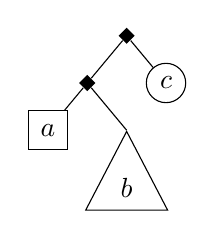
\begin{tikzpicture}[itermtree]
	\node[ap] {} child {
		node[ap] {} child { node[pure] {$a$} } child[subtrm] { node[subtrm] {$b$} }
	} child { node[term] {$c$} };
\end{tikzpicture}
\caption{$(\spure a \sap b) \sap \sterm c$ as a tree.}
\label{fig:iterm-ex}
\end{minipage}\hfill
\begin{minipage}[t]{0.46\textwidth}\centering
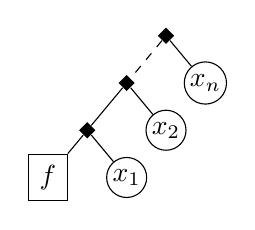
\begin{tikzpicture}[itermtree]
	\node[ap] {} child {
		node[ap] {} child {
			node[ap] {} child {
				node[pure] {$f$}
			} child { node[term] {$x_1$} }
		} child { node[term] {$x_2$} }
	    edge from parent [abbrv]
	} child { node[term] {$x_n$} };
\end{tikzpicture}
\caption{A term in canonical form.}
\label{fig:iterm-nf-ex}
\end{minipage}
\end{figure}

Idiomatic terms are visualized naturally as trees.
This will be helpful in explaining term transformations.
Figure~\ref{fig:iterm-ex} shows the conventions:
Inner nodes correspond to $\sap$, leaves are either pure terms (boxes) or
opaque terms (circles).
Whole subterms may be abbreviated by a triangle.
A term has canonical form if it consists of a single pure node to which a number
of opaque terms (or none) are applied in sequence.
Figure~\ref{fig:iterm-nf-ex} gives a general example.
A formal construction follows:

\begin{definition}[Canonical form]
The set $\mathcal{C} \subset \mathcal{I}$ of idiomatic terms in canonical form
is defined inductively as
\begin{gather}
	\spure x \in \mathcal{C}, \label{eq:cf-base}\\
	t \in \mathcal{C} \implies t \sap \sterm s \in \mathcal{C}. \label{eq:cf-step}
\end{gather}
\end{definition}

\begin{figure}\centering
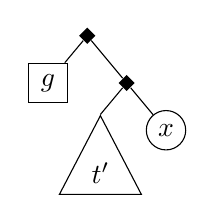
\begin{tikzpicture}[itermtree]
	\node[ap] {} child { node[pure] {$g$} } child {
		node[ap] {} child[subtrmn] { node[subtrm] {$t'$} } child { node[term] {$x$} }
	};
\end{tikzpicture}
\raisebox{10mm}{$\qquad\simeq\qquad$}
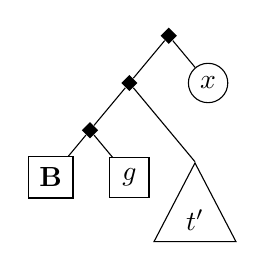
\begin{tikzpicture}[itermtree]
	\node[ap] {} child {
		node[ap] {} child {
			node[ap] {} child { node[pure] {$\mathbf{B}$} } child { node[pure] {$g$} }
		} child[subtrmf] { node[subtrm] {$t'$} }
	} child { node[term] {$x$} };
\end{tikzpicture}
\raisebox{10mm}{$\qquad\simeq\qquad$}
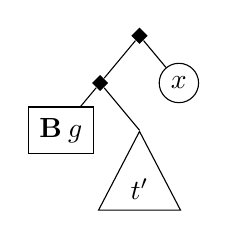
\begin{tikzpicture}[itermtree]
	\node[ap] {} child {
		node[ap] {} child { node[pure] {$\mathbf{B} \sapp g$} } child[subtrm] { node[subtrm] {$t'$} }
	} child { node[term] {$x$} };
\end{tikzpicture}
\caption{The ``pure-rotate'' step.}
\label{fig:pure-rotate}
\end{figure}

It is not entirely obvious how a canonical form can be derived from equations
\eqref{eq:iterm-id}--\eqref{eq:iterm-xchng}.
Rewriting blindly with these is prone to infinite recursion.
Therefore we need a more controlled algorithm.
As we have said before, we use \emph{normal form} to refer to the particular
canonical form derived from those equations.
Consider an idiomatic term $t$.
If $t$ is a single pure term, then it is already in normal form.
The case $t = \sterm x$ is also easy:
Due to \eqref{eq:iterm-id}, we have $t \simeq \spure{(\sabs{x}{x})} \sap t$,
which is in normal form.
But in the case of $t = u \sap v$, various steps could be performed,
depending on the subterms.
We simplify the situation by normalizing each subterm recursively, so we get
an equivalent term $u' \sap v'$ where $u',v' \in \mathcal{C}$.

Now let us assume that $u'$ is just $\spure g$.
If $v'$ is also a pure term, they can be combined along \eqref{eq:iterm-morph}.
Otherwise, the term looks like the one on the left of Figure~\ref{fig:pure-rotate}.
As is shown there, the term tree can be rotated such that one opaque term moves
to the outer-most level.
This is the same equivalence as stated in \eqref{eq:pure-rotate}.
Because the remaining part again has the shape ``pure term applied to normal
form'', we proceed recursively.
In pattern-matching style, the transformation `pure-nf' reads
\begin{align}
	\operatorname{pure-nf}(\spure g \sap (f \sap x)) &=
		\operatorname{pure-nf}{(\spure{(\mathbf{B} g)} \sap f)} \sap x \\
	\operatorname{pure-nf}(\spure f \sap \spure x) &= \spure{(f x)}
\end{align}
\begin{lemma}\label{thm:pure-nf}
For all $g \in \mathcal{T}$ and $t \in \mathcal{C}$,
$\operatorname{pure-nf}(\spure g \sap t)$ is well-defined, and%
\/\footnote{$a \in S \simeq b$ abbreviates ``$a \in S$ and $a \simeq b$''.}
$\operatorname{pure-nf}(\spure g \sap t) \in \mathcal{C} \simeq \spure g \sap t$.
\end{lemma}
\begin{proof}
We prove all claims simultaneously by induction on $t \in \mathcal{C}$,
where $g$ is arbitrary.
\begin{prfcases}
\item Assume $t = \spure x$ for some $x \in \mathcal{T}$.
	Only the second equation applies, so we have
	\[ \operatorname{pure-nf}(\spure g \sap t) = \spure{(g \sapp x)}. \]
	All pure terms are in $\mathcal{C}$, and equivalence follows from
	\eqref{eq:iterm-morph}.
\item Assume $t = t' \sap \sterm x$ for some
	$t' \in \mathcal{C}$, $x \in \mathcal{T}$, and that the hypothesis holds
	for $t'$ and all $g$.
	Only the first equation applies, so
	\[ \operatorname{pure-nf}(\spure g \sap t) =
		\operatorname{pure-nf}(\spure{(\mathbf{B} g)} \sap t') \sap \sterm x. \]
	Instantiating the induction hypothesis, we find that
	\[ \operatorname{pure-nf}(\spure{(\mathbf{B} \sapp g)} \sap t') \in \mathcal{C} \simeq
		\spure{(\mathbf{B} \sapp g)} \sap t' \]
	is well-defined.
	$\mathcal{C}$ is closed under application to opaque terms \eqref{eq:cf-step},
	hence $\operatorname{pure-nf}(\spure g \sap t) \in \mathcal{C}$.
	Finally, we have
	\begin{align*}
		\operatorname{pure-nf}(\spure g \sap t) &\simeq
			\spure{(\mathbf{B} \sapp g)} \sap t' \sap \sterm x \\
		&\stackrel{\mathclap{\eqref{eq:pure-rotate}}}{\simeq}
			\spure g \sap (\spure t' \sap \sterm x) =
			\spure g \sap t. \qedhere
	\end{align*}
\end{prfcases}
\end{proof}

Going back to $u' \sap v'$, we assumed that $u'$ is a pure term.
The case where $v'$ is pure instead can be translated to the former by
\begin{equation}
	\operatorname{nf-pure}(f \sap \spure x) =
		\operatorname{pure-nf}{(\spure{((\sabs{x}\sabs{f}{f x}) \sapp x)} \sap f)} \\
\end{equation}
\begin{lemma}\label{thm:nf-pure}
For all $t \in \mathcal{C}$ and $x \in \mathcal{T}$,
$\operatorname{nf-pure}(t \sap \spure x)$ is well-defined, and
$\operatorname{nf-pure}(t \sap \spure x) \in \mathcal{C} \simeq t \sap \spure x$.
\end{lemma}
\begin{proof}
Follows from Lemma~\ref{thm:pure-nf} and \eqref{eq:iterm-xchng}.
\end{proof}

\begin{figure}\centering
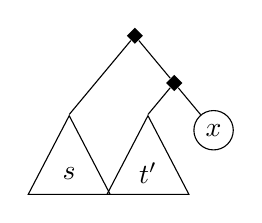
\begin{tikzpicture}[itermtree]
	\node[ap] {} child[subtrmf] { node[subtrm] {$s$} } child {
		node[ap] {} child[subtrmn] { node[subtrm] {$t'$} } child { node[term] {$x$} }
	};
\end{tikzpicture}
\raisebox{10mm}{$\qquad\simeq\qquad$}
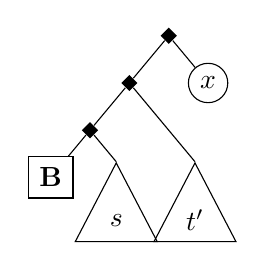
\begin{tikzpicture}[itermtree]
	\node[ap] {} child {
		node[ap] {} child {
			node[ap] {} child { node[pure] {$\mathbf{B}$} } child[subtrmn] {
				node[subtrm] {$s$}
			}
		} child[subtrmf] { node[subtrm] {$t'$} }
	} child { node[term] {$x$} };
\end{tikzpicture}
\caption{The ``rotate'' step.}
\label{fig:rotate}
\end{figure}

Finally, we look at general $u'$, $v'$.
A term rotation is useful again, see Figure~\ref{fig:rotate}.
Before recursion, we must normalize the subterm $\spure \mathbf{B} \sap s$.
But we already know how to do this: by `pure-nf'.
The base case is reached when $v'$ is a single pure term, which is the domain
of `nf-pure'.
The corresponding transformation is therefore
\begin{align}
	\operatorname{nf-nf}(g \sap (f \sap x)) &=
		\operatorname{nf-nf}{(\operatorname{pure-nf}{(\spure \mathbf{B} \sap g)} \sap f)} \sap x \label{eq:nf-nf1}\\
	\operatorname{nf-nf}(t) &= \operatorname{nf-pure}(t) \quad\text{(otherwise)}
\end{align}
\begin{lemma}\label{thm:nf-nf}
For all $s,t \in \mathcal{C}$,
$\operatorname{nf-nf}(s \sap t)$ is well-defined, and
$\operatorname{nf-nf}(s \sap t) \in \mathcal{C} \simeq s \sap t$.
\end{lemma}
\begin{proof}
The proof is similar to the one of Lemma~\ref{thm:pure-nf}, by induction on
$t \in \mathcal{C}$ and arbitrary $s \in \mathcal{C}$.
\begin{prfcases}
\item Assume $t = \spure x$ for some $x \in \mathcal{T}$.
	The second equation applies, so we have
	\[ \operatorname{nf-nf}(s \sap t) = \operatorname{nf-pure}(s \sap \spure x). \]
	Since $s \in \mathcal{C}$, the claim follows directly from Lemma~\ref{thm:nf-pure}.
\item Assume $t = t' \sap \sterm x$ for some
	$t' \in \mathcal{C}$, $x \in \mathcal{T}$, and that the hypothesis holds
	for $t'$ and all $s \in \mathcal{C}$.
	Only the first equation applies,
	\[ \operatorname{nf-nf}(s \sap t) =
		\operatorname{nf-nf} (\operatorname{pure-nf}(\spure \mathbf{B} \sap s) \sap t') \sap \sterm x. \]
	We have
	$\operatorname{pure-nf}(\spure \mathbf{B} \sap s) \in \mathcal{C} \simeq \spure \mathbf{B} \sap s$
	from Lemma~\ref{thm:pure-nf}.
	Thus we can instantiate the induction hypothesis, and the transformed term
	is indeed in normal form.
	Furthermore,
	\begin{align*}
		\operatorname{nf-nf}(s \sap t) &\stackrel{\mathclap{\text{(IH)}}}{\simeq}
			\operatorname{pure-nf}(\spure \mathbf{B} \sap s) \sap t' \sap \sterm x \\
		&\simeq \spure \mathbf{B} \sap s \sap t' \sap \sterm x \\
		&\stackrel{\mathclap{\eqref{eq:iterm-comp}}}{\simeq}
			s \sap (t' \sap \sterm x) = s \sap t. \qedhere
	\end{align*}
\end{prfcases}
\end{proof}

\begin{algorithm}[t]
\caption{Normalization of idiomatic terms.}
\label{alg:normalize}
\begin{gather*}
	\begin{align*}
		\operatorname{normalize}(\spure x) &= \spure x \\
		\operatorname{normalize}(\sterm x) &= \spure{(\sabs{x}{x})} \sap \sterm x \\
		\operatorname{normalize}(x \sap y) &=
			\operatorname{nf-nf}(\operatorname{normalize} x \sap \operatorname{normalize} y)
	\end{align*} \\[2ex]
	\begin{align*}
		\operatorname{nf-nf}(g \sap (f \sap x)) &=
			\operatorname{nf-nf}{(\operatorname{pure-nf}{(\spure \mathbf{B} \sap g)} \sap f)} \sap x \\
		\operatorname{nf-nf}(t) &= \operatorname{nf-pure}(t) \quad\text{(otherwise)}
	\end{align*} \\[2ex]
	\begin{align*}
		\operatorname{pure-nf}(\spure g \sap (f \sap x)) &=
			\operatorname{pure-nf}{(\spure{(\mathbf{B} g)} \sap f)} \sap x \\
		\operatorname{pure-nf}(\spure f \sap \spure x) &= \spure{(f x)}
	\end{align*} \\[2ex]
	\operatorname{nf-pure}(f \sap \spure x) =
		\operatorname{pure-nf}{(\spure{((\sabs{x}\sabs{f}{f x}) \sapp x)} \sap f)}
\end{gather*}
\end{algorithm}

Algorithm~\ref{alg:normalize} summarizes all pieces of the normal form
transformation.
`normalize' is the entry point and performs the main recursion mentioned in the
beginning.
We haven't proved the desired property for `normalize' yet, but this is just a
straightforward induction.

\begin{lemma}\label{thm:normalize}
For all $t \in \mathcal{I}$, $\operatorname{normalize} t$ is well-defined, and
$\operatorname{normalize} t \in \mathcal{C} \simeq t$.
\end{lemma}
\begin{proof}
By induction on $t$, Lemma~\ref{thm:nf-nf}, and equation \eqref{eq:iterm-id}.
\end{proof}

At this point, we know that it is always possible to obtain a certain canonical
form.
This is not sufficient to setup the complete proving process, though.
We need to learn a bit more about the structure of idiomatic terms and how it
relates to lifting.

\begin{definition}[Opaque subterms]\label{def:opaque-seq}
The sequence of opaque subterms of an idiomatic term is defined by the
recursive function
\[
	\operatorname{opaq}(\spure x) = [], \quad
	\operatorname{opaq}(\sterm x) = [x], \quad
	\operatorname{opaq}(s \sap t) = \operatorname{opaq} s @ \operatorname{opaq} t.
\]
$@$ denotes concatenation of lists.
\end{definition}

\begin{definition}[Unlifting]\label{def:unlifting}
Let $t$ be some idiomatic term, and $n = |\operatorname{opaq} t|$.
Let $v_{i \in \{1..n\}}$ be new variable symbols that do not occur anywhere in
$t$.
The ``unlifted'' lambda term corresponding to $t$ is defined as
\[ \unlift{t} = \sabs{v_1} \cdots \sabs{v_n}{\operatorname{vary}_1 t}, \]
where
\begin{align}
	\operatorname{vary}_i (\spure x) &= x, \\
	\operatorname{vary}_i (\sterm x) &= v_i, \\
	\operatorname{vary}_i (s \sap t) &=
		(\operatorname{vary}_i s) \sapp (\operatorname{vary}_{i + |\operatorname{opaq} s|} t).
\end{align}
\end{definition}

\begin{example}\label{exmp:unlift}
The definition of $\downarrow$ may need some explanation.
Consider the idiomatic term
\[ t \equiv \spure{f} \sap x \sap (\spure{g} \sap y \sap z). \]
Its unlifted term is
\[ \unlift{t} = \sabs{a}\sabs{b}\sabs{c}{f \sapp a \sapp (g \sapp b \sapp c)}. \]
The applicative structure is the same, but all opaque terms have been
substituted for new bound variables, which are assigned from left to right.
We do not define lifting formally here, but it should be clear that this is
some sort of inverse operation, given that variables appear only once.
\end{example}

The interesting properties about these two concepts is that they are preserved
by the equivalence relation $\simeq$, and can be directly read from the
canonical form.
Furthermore, we can leverage them to show the uniqueness of the normal form.

\begin{lemma}\label{thm:unlift-equiv}
For equivalent terms $s \simeq t$, the sequences of opaque terms are equivalent
w.r.t $\termeq$, and $\unlift{s} \termeq \unlift{t}$.
\end{lemma}
\begin{proof} (Sketch.)
By induction on the relation $s \simeq t$, where we show
$\operatorname{vary}_i s \termeq \operatorname{vary}_i t$ instead.
The index $i$ is arbitrary.
The part regarding opaque terms is shown easily for each case:
We note that in \eqref{eq:iterm-id}--\eqref{eq:iterm-xchng}, the opaque terms
are identical for both sides.
By the induction hypothesis, this is also true for the necessary closure rules
for symmetry, transitivity, and substitution.
It is obvious that \eqref{eq:termeq-lift} also preserves opaque terms.
Regarding unlifted terms, we have
\begin{prfcases}
\item \eqref{eq:iterm-id}
	\[ \operatorname{vary}_i (\spure{(\sabs{x}{x})} \sap x) =
		(\sabs{x}{x}) \sapp (\operatorname{vary}_i x) \termeq \operatorname{vary}_i x. \]
\item \eqref{eq:iterm-comp}
	Let $j = i + |\operatorname{opaq} g|$ and $k = j + |\operatorname{opaq} f|$.
	\begin{align*}
		\operatorname{vary}_i (\spure \mathbf{B} \sap g \sap f \sap x) &=
		\mathbf{B} \sapp (\operatorname{vary}_i g) \sapp (\operatorname{vary}_j f) \sapp (\operatorname{vary}_k g) \\
		&\termeq (\operatorname{vary}_i g) \sapp ((\operatorname{vary}_j f) \sapp (\operatorname{vary}_k g)) \\
		&= \operatorname{vary}_i (g \sap (f \sap x)).
	\end{align*}
\item \eqref{eq:iterm-morph} and \eqref{eq:iterm-xchng} are similar.
\item \eqref{eq:termeq-lift} By induction.
\item Symmetry, transitivity, and substitution: These follow from the induction
	hypothesis and the corresponding properties of $\termeq$.
\end{prfcases}
\end{proof}

\begin{lemma}\label{thm:unlift-head}
Let $\spure f$ be the single pure term in $t \in \mathcal{C}$.
Then $f \termeq \unlift{t}$.
\end{lemma}
\begin{proof}
By induction on $\mathcal{C}$.
The base case is trivial.
For the step case, we need to prove that
\[ f' \termeq \unlift{(g \sap \sterm x)} =
	\sabs{v_1} \dots \sabs{v_n} \sabs{v_{n+1}}{(\operatorname{vary}_1 g) \sapp v_{n+1}}, \]
where $\spure f'$ is the single pure term in $g$, $n = |\operatorname{opaq} g|$,
and $v_i$ are new variables.
The right-hand side can be eta-reduced to
\[ \sabs{v_1} \dots \sabs{v_n}{(\operatorname{vary}_1 g)} = \unlift{g}. \]
From the induction hypothesis we get $f' \termeq \unlift{g}$, which
concludes the proof.
\end{proof}

This lemma is why we need eta-equivalence and not just use $=_{\alpha\beta}$.
In fact, we can find a counterexample of equivalent canonical forms that do
not agree in the pure function if $\to_\eta$ is not available:
\[ \spure{(\sabs{x}{x})} \sap (\spure f \sap x) \simeq
	\spure f \sap x \simeq \spure{(\sabs{x}{f \sapp x})} \sap x. \]
The middle term is derived from \eqref{eq:iterm-id}, the latter from
\eqref{eq:iterm-comp}.

\begin{corollary}\label{thm:nf-unique}
The normal form is structurally unique.
Formally, if $s,t \in \mathcal{C}$ and $s \simeq t$, then $s \termeq t$.
\end{corollary}

Now we have all tools ready to complete the picture.
The following theorem shows that (limited) lifting is possible with just
the applicative laws.
Its proof hints towards the implementation in Isabelle, which is of course
based on the normal form:
Under the condition that the opaque terms are equivalent, normalizing two
idiomatic terms reduces the problem to the ``unlifted'' terms.

\begin{theorem}\label{thm:nf-lifting}
Let $s,t \in \mathcal{I}$ with $\operatorname{opaq} s \termeq \operatorname{opaq} t$.
If $\unlift{s} \termeq \unlift{t}$ (the base equation), then $s \simeq t$.
\end{theorem}
\begin{proof}
From Lemma~\ref{thm:normalize} we obtain normal forms $s' \simeq s$ and
$t' \simeq t$.
With the base equation and Lemma~\ref{thm:unlift-equiv} we get
$\unlift{s'} \termeq \unlift{t'}$.
By Lemma~\ref{thm:unlift-head} and the condition on the opaque subterms, it
follows that $s' \termeq t'$ and further $s \simeq t$.
\end{proof}

\subsection{Implementation}\label{subsec:nf-implementation}  % TODO title?

We introduced an algorithm for computing the normal form of an idiomatic term,
and argued for its central role in lifting.
In order to be useful in the context of theorem proving, just providing the
normal form is not sufficient.
We need to establish a formal proof of the equivalence.
In Isabelle, this means constructing a theorem $t = t'$, where $t'$ is the
normal form of $t$.
We observe that in Algorithm~\ref{alg:normalize} each equation can be recast
in the following way:
The input term is first transformed in a fixed way that changes the outermost
constitution.
Then, the whole term or subterms thereof are substituted by other functions%
---or recursively---, possibly multiple times.
For instance, in the first equation \eqref{eq:nf-nf1} for nf-nf, the term
$g \sap (f \sap x)$ (where $g$, $f$, $x$ should be understood as placeholders
for concrete terms) is rearranged to $\spure \mathbf{B} \sap g \sap f \sap x$.
The subterm $\spure \mathbf{B} \sap g$ is passed to pure-nf and replaced by
the result, say $g'$.
nf-nf acts on $g' \sap f$, yielding $f'$, such that the final term is
$f' \sap x$.

\begin{table}[t]\centering\small
\begin{tabular}{lrcll}
Function & Pattern & & Substitution & Name \\
\hline
normalize & $\sterm x$ & $\simeq$ & $\spure{(\sabs{x}{x})} \sap \sterm x$ \\
	& $\svar{x}$ & $=$ & $\pure{(\abs{x}{x})} \ap \svar{x}$ & \texttt{I\_intro} \\[1ex]
nf-nf & $g \sap (f \sap x)$ & $\simeq$ & $\spure \mathbf{B} \sap g \sap f \sap x$ \\
	& $\svar{g} \ap (\svar{f} \ap \svar{x})$ & $=$ & $\pure{(\abs{g f x}{g (f x)})} \ap \svar{g} \ap \svar{f} \ap \svar{x}$ & \texttt{B\_intro} \\[1ex]
pure-nf & $\spure g \sap (f \sap x)$ & $\simeq$ & $\spure{(\mathbf{B} \sapp g)} \sap f \sap x$ \\
	& $\pure \svar{g} \ap (\svar{f} \ap \svar{x})$ & $=$ & $\pure{(\abs{f x}{\svar{g} (f x)})} \ap \svar{f} \ap \svar{x}$ & \texttt{B\_pure} \\[1ex]
pure-nf & $\spure f \sap \spure x$ & $\simeq$ & $\spure{(f \sapp x)}$ \\
	& $\pure \svar{f} \ap \pure \svar{x}$ & $=$ & $\pure{(\svar{f} \svar{x})}$ & \texttt{merge} \\[1ex]
nf-pure & $f \sap \spure x$ & $\simeq$ & $\spure{((\sabs{x}{\sabs{f}{f \sapp x}}) \sapp x)} \sap f$ \\
	& $\svar{f} \ap \pure \svar{x}$ & $=$ & $\pure{(\abs{f}{f \svar{x}})} \ap \svar{f}$ & \texttt{swap}
\end{tabular}
\caption{Fixed transformations of Algorithm~\ref{alg:normalize}, with
corresponding rewrite rules. Identity cases are omitted.}
\label{tab:normalize-rules}
\end{table}

Table~\ref{tab:normalize-rules} shows all initial transformations.
It is no coincidence that these are the well-known equivalences
\eqref{eq:iterm-id}--\eqref{eq:iterm-xchng} and~\eqref{eq:pure-rotate}, which
were used in the correctness proofs.
Each transformation has been augmented with the corresponding HOL equation.
The mapping from syntactic idiomatic terms to HOL terms is obvious;
$\pure$ and $(\ap)$ are the concrete constants of the idiom under consideration.
The variables standing for arbitrary opaque terms become new schematic variables,
representing unknowns which may be instantiated.
%$\mathbf{B}$ has been unfolded, ...
Rule \texttt{B\_pure} is easily proven by rewriting with \texttt{B\_intro} and
\texttt{merge}.
The other rules are the applicative laws and thus are available from the
registration infrastructure, see also \todo. % TODO ref to design section
Applying a transformation to a term means instantiating the rule such that the
left hand side is equal to that term.
Isabelle provides a low-level reasoning framework for combining \emph{conversions}~
\cite{paulson83}, which we use here.
A conversion is a function which takes a term $t$ and returns a theorem
$t = u$ for some $u$.%
\footnote{Isabelle's conversions use the Pure equality $\equiv$.}
The ML function \verb+Conv.rewr_conv+ turns a proven equation into such a
conversion function.
When the resulting conversion is applied, it attempts to instantiate the
schematic variables in the equation.
Note that conversions can fail; here if there is no match.
Basic conversion combinators are the \verb+then_conv+ operator, which chains
two conversions sequentially (and fails if any of these does),
and the \verb+else_conv+ operator, which attempts to apply the first conversion,
but uses the second if the first fails.
%\verb+Conv.all_conv+ is the identity of \verb+then_conv+; ...
Because rewrite conversions act like pattern matching guards, we combine them
with \verb+else_conv+ to recreate the case switching of the algorithm.
Combinators like \verb+Conv.arg1_conv+ facilitate the rewriting of subterms---%
this one takes a conversions and modifies it such that it applies to the left
operand of a binary operator.
With these tools at hand, we can construct the normal form conversion.
The recursive pieces can be expressed just as recursive auxiliary functions.
However, we lose a bit of generality by using \verb+Conv.arg1_conv+ to access
the left operand of $(\ap)$, because it requires that $(\ap)$ is not a
beta-redex.
This could be solved by creating a specialized combinator, which does pattern
matching instead of simple term deconstruction.

\begin{figure}
\begin{lstlisting}[language=ml]
fun normalform_conv ctxt af =
  let
    val rules = facts_of_afun af;

    val leaf_conv = rename_rewr_conv (fn t => [("x", term_to_vname t)])
      (#I_intro rules);
    val merge_conv = Conv.rewr_conv (#merge rules);
    val swap_conv = Conv.rewr_conv (#swap rules);
    val rotate_conv = rename_rr_conv "x" (#B_intro rules);
    val pure_rotate_conv = rename_rr_conv "x" (#B_pure rules);

    fun normalize_pure_nf ct = ((pure_rotate_conv then_conv
      Conv.arg1_conv normalize_pure_nf) else_conv merge_conv) ct;
    val normalize_nf_pure = swap_conv then_conv normalize_pure_nf;
    fun normalize_nf_nf ct = ((rotate_conv then_conv
        Conv.arg1_conv (Conv.arg1_conv normalize_pure_nf then_conv
          normalize_nf_nf)) else_conv
      normalize_nf_pure) ct;

    fun normalize ct =
      let val t = Thm.term_of ct
      in if can (dest_comb ctxt af) t
        then (Conv.arg1_conv normalize then_conv
            Conv.arg_conv normalize then_conv normalize_nf_nf) ct
        else if can (dest_pure ctxt af) t
          then Conv.all_conv ct
          else leaf_conv ct
      end;
  in normalize end;
\end{lstlisting}
\caption{ML implementation of normalization.}
\label{fig:ml-normalform}
\end{figure}

Figure~\ref{fig:ml-normalform} shows the ML code.
It is parameterized by the applicative functor \verb+af+, which contains all
the necessary rules.
In the helper function \verb+normalize+, the different cases are selected
by predicates like \verb+can (dest_comb ctxt af) t+, which is true only if
term \verb+t+ fits the pattern $\_ \ap_\mathtt{af} \_$.
We do this here because it is the only recursive conversion which is not
guarded by a rewrite rule before recurring, so we want to protect against
rampant rewriting.
Finally, \verb+rename_rewr_conv+ and \verb+rename_rr_conv+ (not shown)
adjust the names of bound variables in the argument rule to the term to convert.
While these names are only hints in Isabelle and obviously subject to alpha
conversion, they influence the display of the proof state.
To elaborate, consider a HOL term $p \ap (q \ap r)$.
Without the adjustment, the normal form would be
$\pure{(\abs{xx_ax_b}{x(x_ax_b)})} \ap p \ap q \ap r$.
The name component $x$ stems from the lambda abstraction in rule \verb+B_intro+.
If the term is part of an equation, the variables of the reduced base equation
will also be called $x$, $x_a$, and $x_b$.
This creates unnecessary confusion, and to help the user, we try to preserve the
variable names of the input term.

\printbibliography

\end{document}
